\section{Additional Figures}
\label{supp:figures}

\textit{Purpose of this supplement.}\;
This supplement collects supplementary figures referenced in the
main text: the coupling-slope forest plot, the rank-inversion
histogram, the per-encoder KB-audit metric profiles, the
RoBERTa-base reference cell, and the KB-argmax-accuracy
distribution by configuration cell.

\subsection{Coupling-slope forest plot}

\begin{figure}[H]
\centering
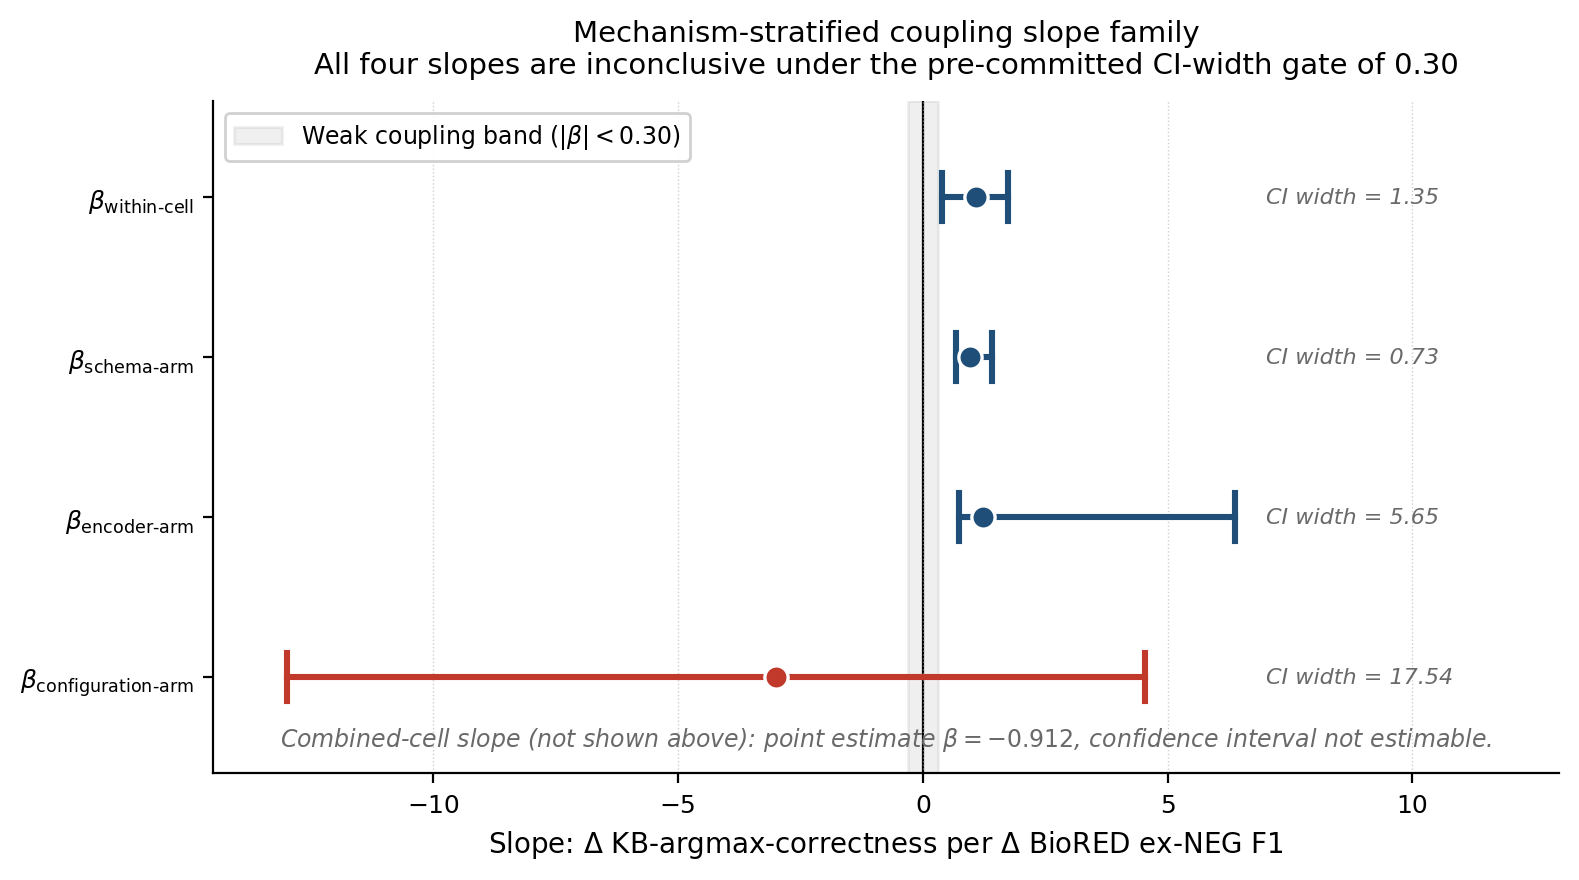
\includegraphics[width=0.92\textwidth]{figures/fig_S2_slope_forest.png}
\caption{Coupling-slope estimates.}
\label{fig:s1-slopes}
\end{figure}

The point estimates are plotted on the natural slope scale (units of
$\Delta$KB argmax accuracy per $\Delta$BioRED ex-NEG F1) with 95\%
cluster-bootstrap confidence intervals. The configuration-arm slope
(red) has a CI spanning both signs; the within-cell, schema-arm, and
encoder-arm slopes (blue) are positive but their CIs all exceed the
0.30 reportability gate. The shaded band marks the $|\beta| < 0.30$
weak-coupling region from the slope-magnitude partition. The
combined-cell slope (point estimate $\beta = -0.91$, CI not estimable)
is noted at the figure's bottom margin. None of the five slopes
reaches a qualitative label (the four with estimable CIs exceed the
0.30-width gate; the fifth has no estimable CI).

\subsection{Rank-inversion histogram}

\begin{figure}[H]
\centering
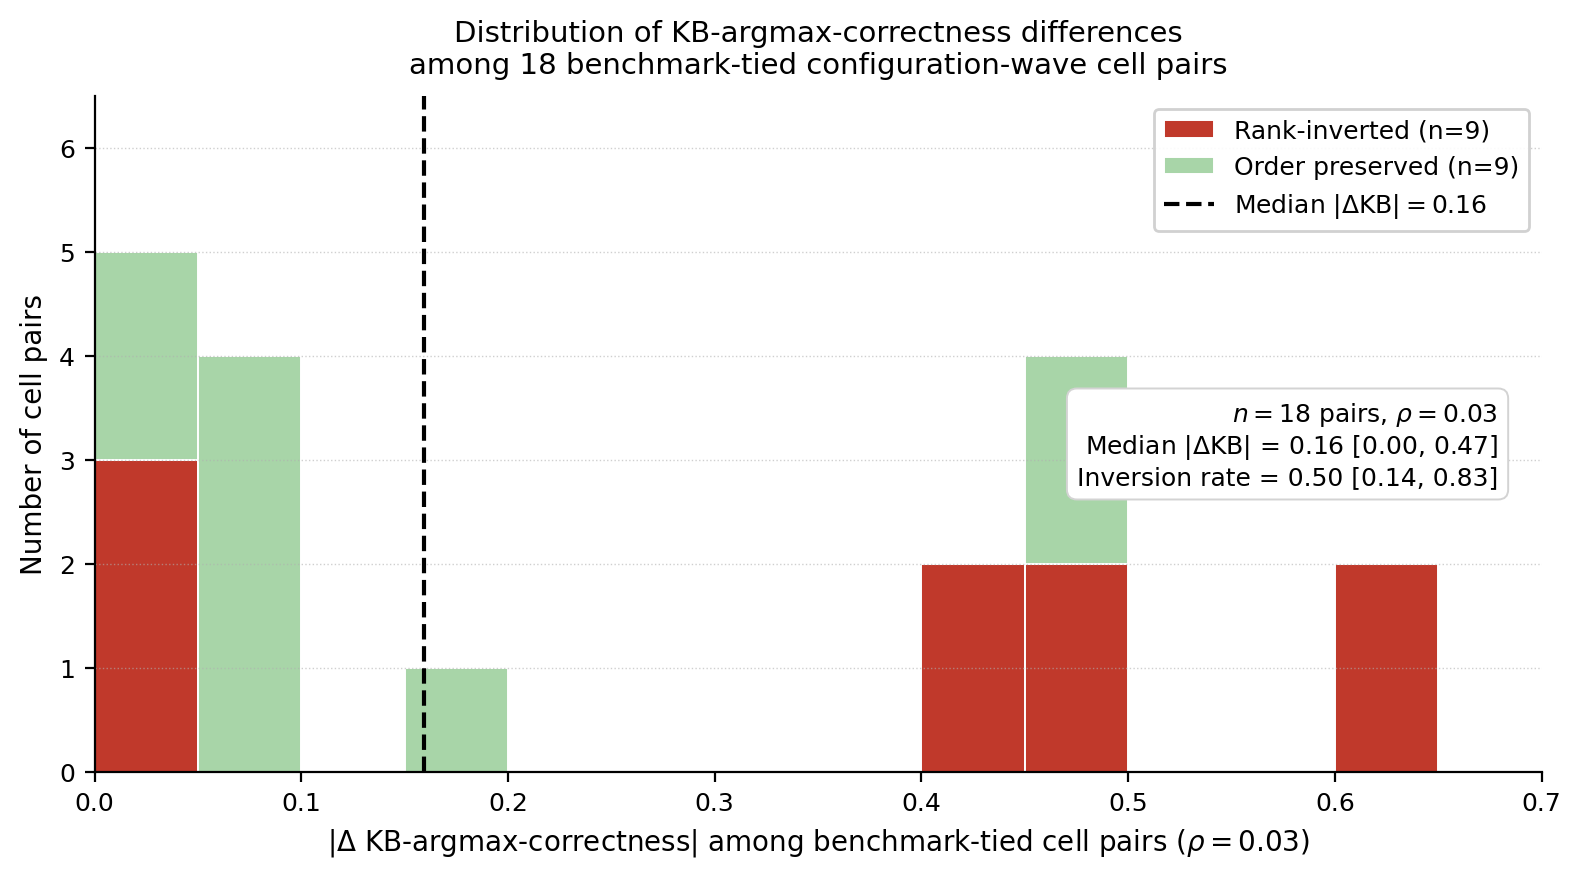
\includegraphics[width=0.92\textwidth]{figures/fig_S3_ordinal_histogram.png}
\caption{$|\Delta\text{KB}|$ distribution among benchmark-tied pairs.}
\label{fig:s2-histogram}
\end{figure}

The histogram shows $|\Delta\text{KB argmax accuracy}|$ across the
18 benchmark-tied configuration-wave cell pairs ($\rho = 0.03$).
Stacked bars distinguish the 9 rank-inverted pairs (red) from the
9 order-preserved pairs (green). The dashed line marks the median
$|\Delta\text{KB}| = 0.16$. The distribution is bimodal: most pairs
cluster either below 0.10 or above 0.40, with the middle of the
range sparsely populated. Both tails contain rank-inverted pairs.

\subsection{Per-encoder KB-audit metric profiles}

\begin{figure}[H]
\centering
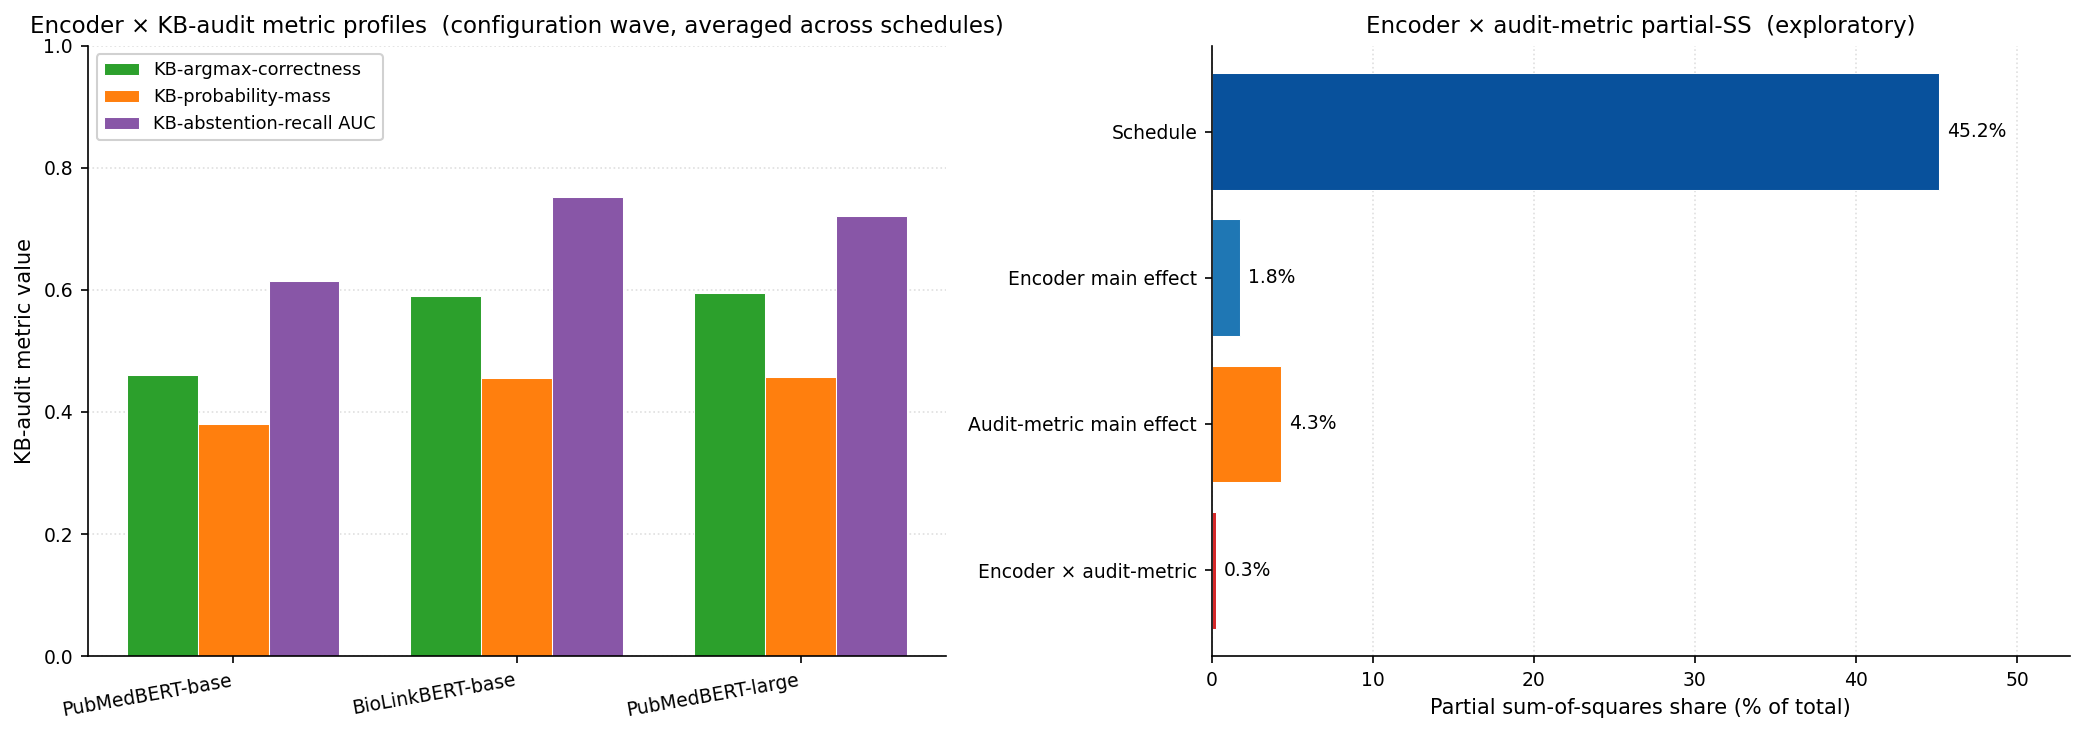
\includegraphics[width=\textwidth]{figures/fig3_kb_surfacing.png}
\caption{Per-encoder KB-audit metric profiles across the three
audit metrics.}
\label{fig:s4-kb-profiles}
\end{figure}

For each biomedical encoder (PubMedBERT-base, BioLinkBERT-base,
PubMedBERT-large) and the RoBERTa-base reference, bars give the
configuration-wave mean of KB argmax accuracy, KB truth
probability, and KB selective-recall AUC under the staged schedule.
The metric ordering of encoders is the same on all three:
BioLinkBERT-base $\approx$ PubMedBERT-large $>$ PubMedBERT-base.
RoBERTa-base trails on KB argmax accuracy and KB truth probability
but is closer on KB selective-recall AUC, consistent with the
abstain-when-uncertain calibration that the AUC metric rewards.

\subsection{RoBERTa-base reference cell}

\begin{figure}[H]
\centering
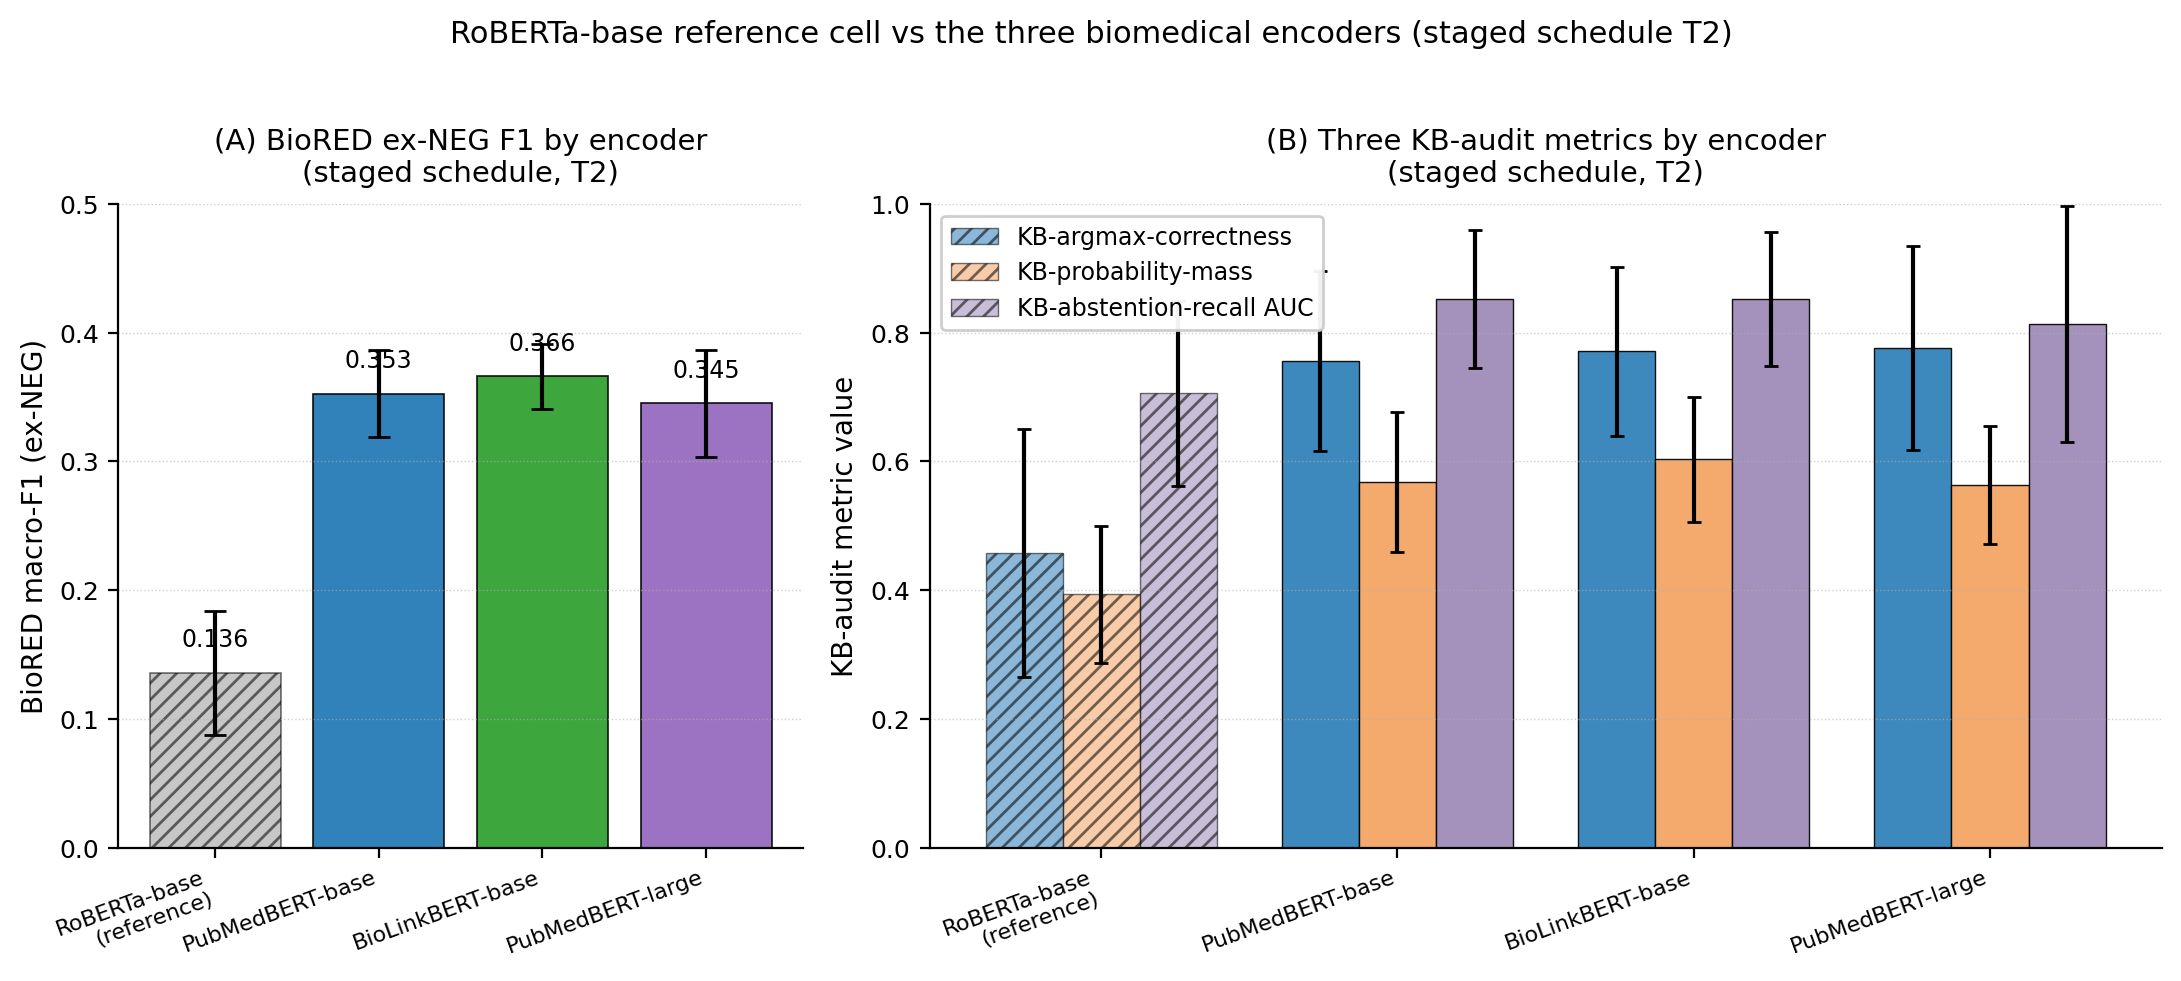
\includegraphics[width=\textwidth]{figures/fig_S4_roberta_reference.png}
\caption{RoBERTa-base reference cell on the staged schedule.}
\label{fig:s3-roberta}
\end{figure}

Bars are means over seeds (RoBERTa-base $n = 10$; biomedical encoders
$n = 20$). Hatched bars mark the RoBERTa-base reference. Panel A
shows BioRED ex-NEG F1: RoBERTa-base trails clearly (0.136 vs
$\sim 0.35$ for the biomedical encoders), confirming a
biomedical-pretraining premium on the BioRED benchmark. Panel B
shows the three KB-audit metrics: the gap is metric-dependent.
RoBERTa-base trails on KB argmax accuracy (0.46 vs $\sim 0.77$)
and on KB truth probability (0.39 vs $\sim 0.58$) but is more
competitive on KB selective-recall AUC (0.71 vs $\sim 0.83$).
The reference cell does not enter any pre-registered hypothesis test.

\subsection{KB argmax accuracy distribution by configuration cell}

\begin{figure}[H]
\centering
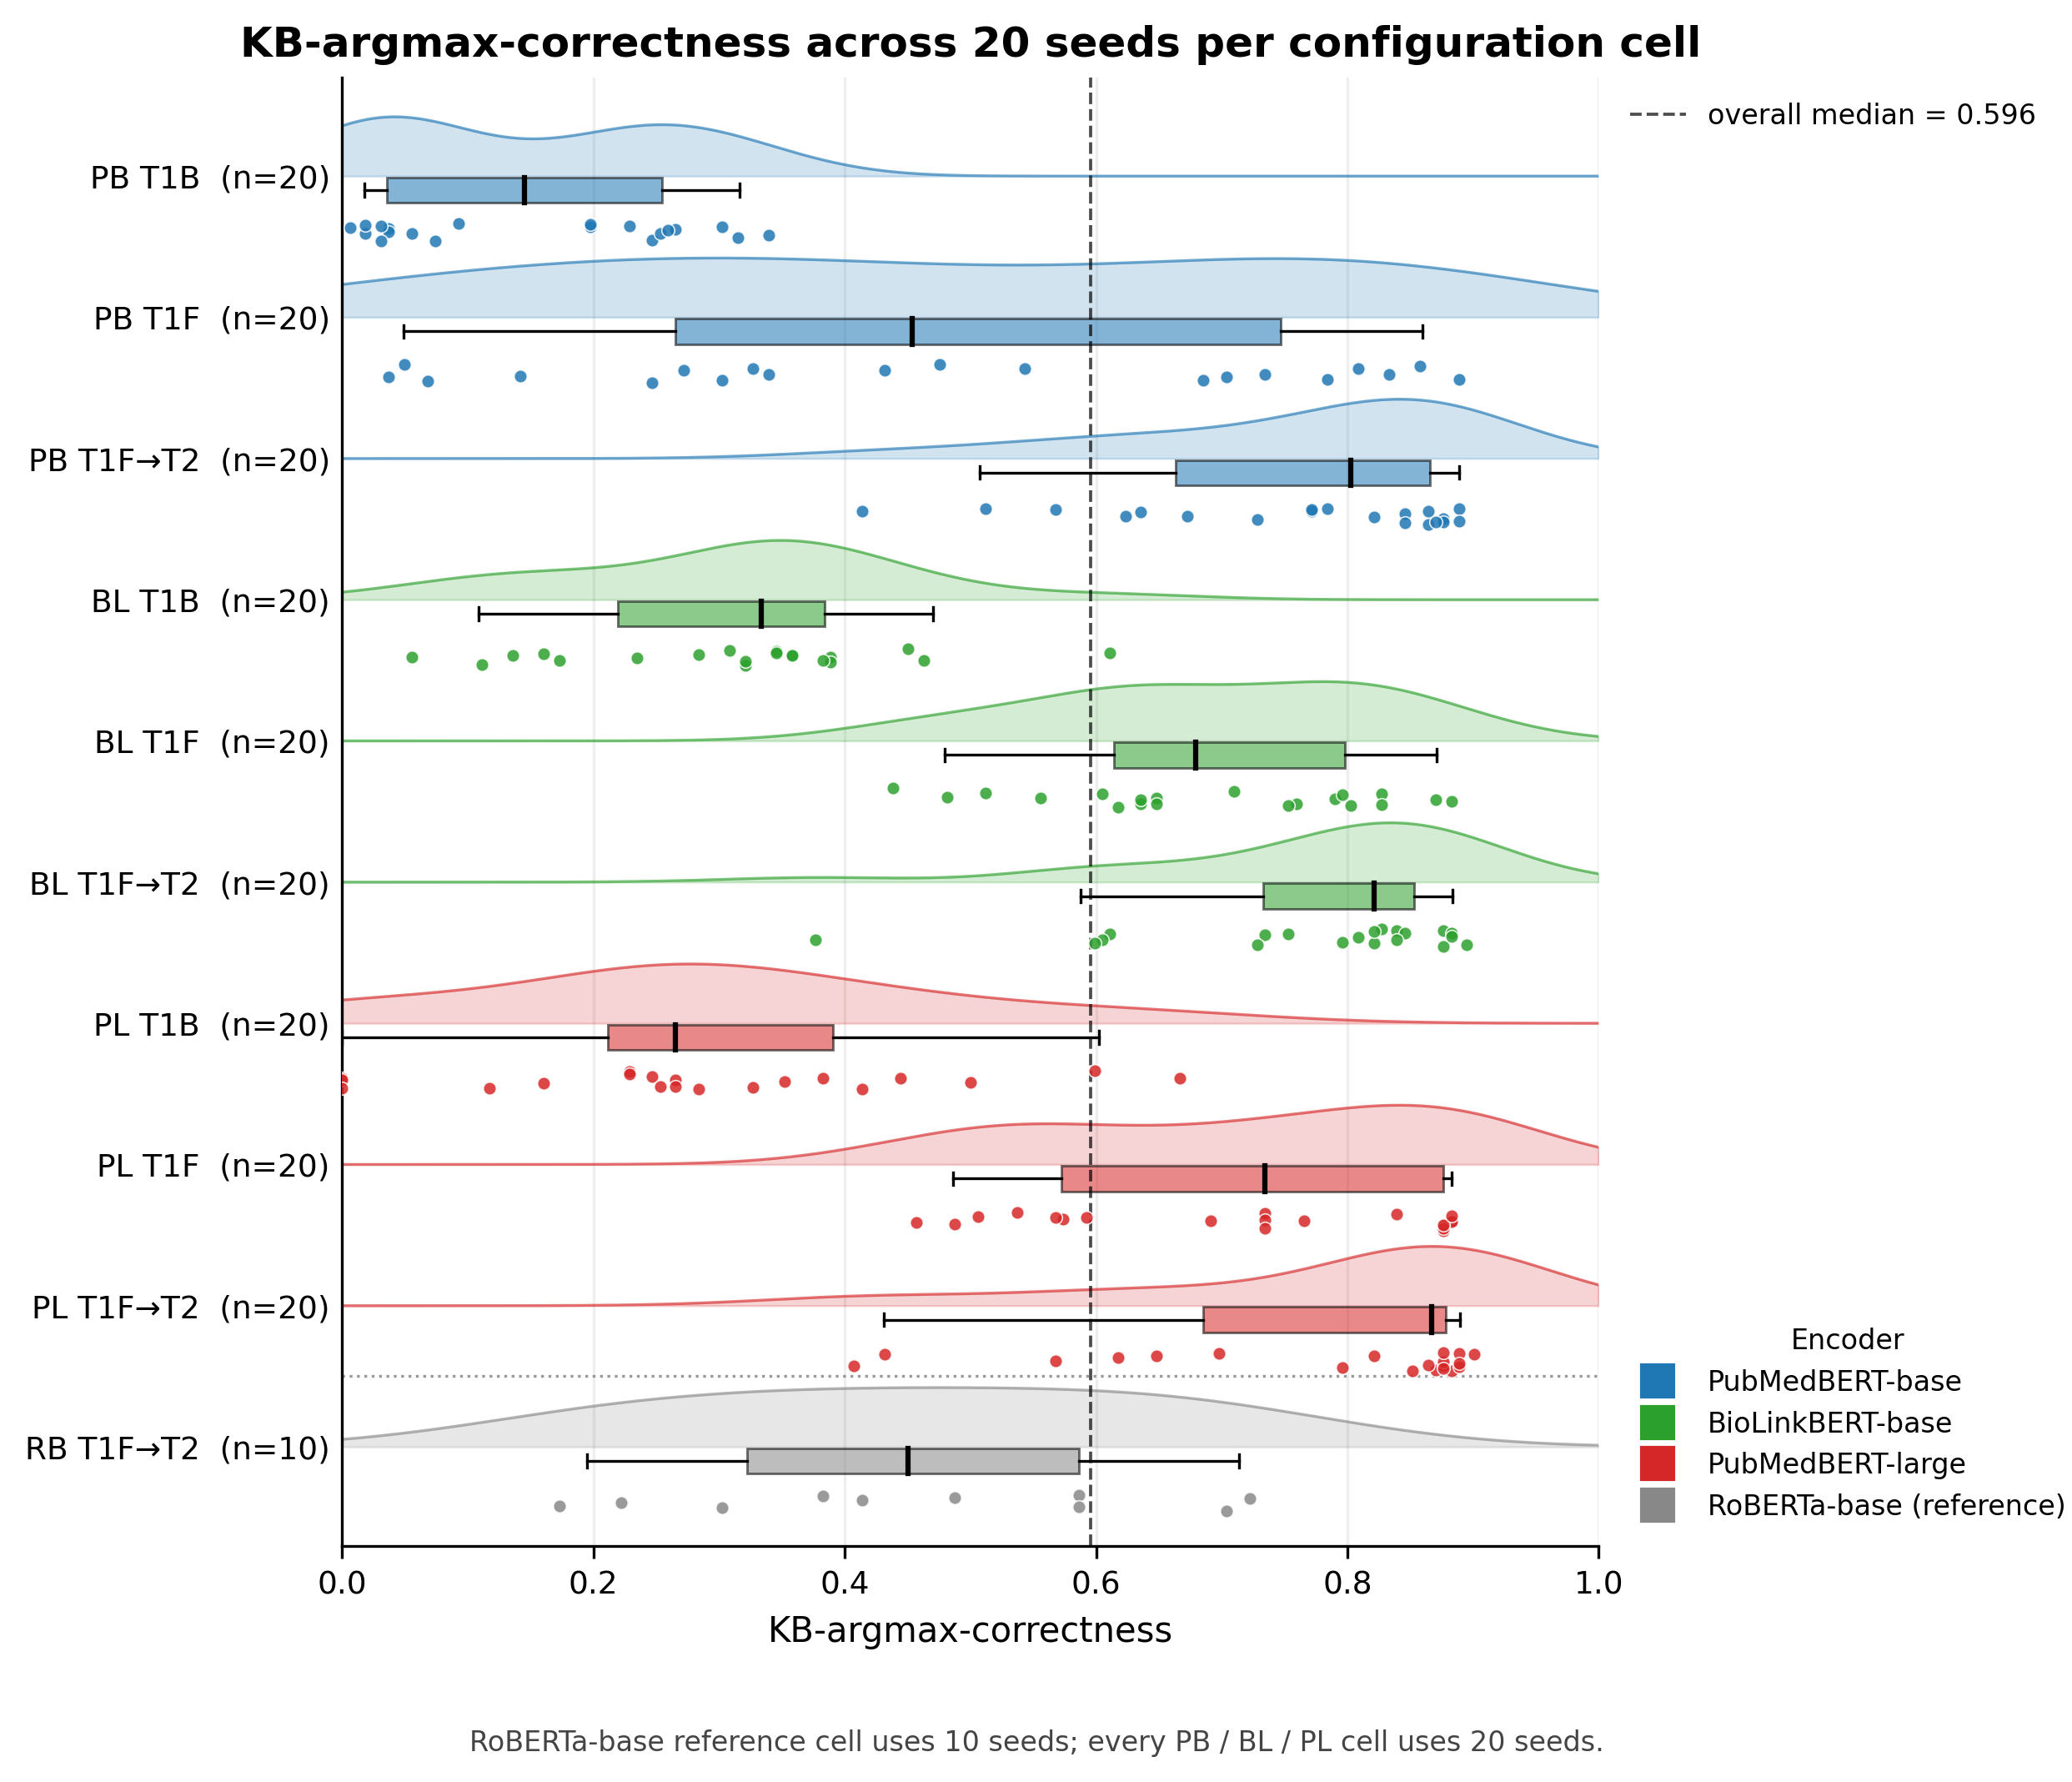
\includegraphics[width=\textwidth]{figures/fig_supp_kb_argmax_distribution.png}
\caption{Seed-level KB argmax accuracy distribution per
configuration-wave cell. Each row corresponds to one
(encoder, schedule) cell; within a row, the half-violin is a
Gaussian kernel-density estimate over the cell's seeds, the box
plot shows 5th--95th percentile whiskers with an interquartile
range box, and the strip shows individual per-seed cell-mean
correctness (each point is one seed's mean over the 162 evaluable
CIViC targets). The vertical dashed line marks the overall median
across all configuration-wave runs; the dotted horizontal line
above the RoBERTa-base row separates the reference cell ($n=10$
seeds) from the main factorial ($n=20$ seeds per cell). Several
cells (notably PB$\,\times\,$T1B and PL$\,\times\,$T1B) show
visibly bimodal seed distributions, consistent with within-cell
mode-collapse at the realised reliability ceiling reported in
\S\ref{sec:stats}: a fraction of seeds within these cells fail to escape
low-KB optima within the pre-registered training budget. Cell
labels: PB = PubMedBERT-base; BL = BioLinkBERT-base;
PL = PubMedBERT-large; RB = RoBERTa-base; T1B = single-corpus
baseline; T1F = multi-corpus flat schedule; T1F$\rightarrow$T2 =
multi-corpus then oncology-projected staged.}
\label{fig:s5-kb-dist}
\end{figure}

\paragraph{Per-family KB breakdown.}
A per-CIViC-entity-pair-family breakdown was considered for this
supplement but omitted: with 162 evaluable targets, the smaller
family (variant--disease, 8 targets) has effective sample size
below 10 under any encoder $\times$ schedule slicing. Per-family
KB performance is recoverable from the per-target KB output in the
released code repository.